\documentclass[sigconf]{acmart}
\AtBeginDocument{%
  \providecommand\BibTeX{{%
    \normalfont B\kern-0.5em{\scshape i\kern-0.25em b}\kern-0.8em\TeX}}}

%% Rights management information.  This information is sent to you
%% when you complete the rights form.  These commands have SAMPLE
%% values in them; it is your responsibility as an author to replace
%% the commands and values with those provided to you when you
%% complete the rights form.
% \setcopyright{none}
\setcopyright{acmcopyright}
\copyrightyear{2021}
\acmYear{2021}
\acmDOI{XXXXXXX.XXXXXXX}

%% These commands are for a PROCEEDINGS abstract or paper.
\acmConference[EE 475 Au '21]{Embedded Systems Capstone}{Dec 13, 2021}{Seattle, WA}
\acmPrice{4.20}
\acmISBN{978-1-4503-XXXX-X/18/06}


%%
%% end of the preamble, start of the body of the document source.
\begin{document}

%%
%% The "title" command has an optional parameter,
%% allowing the author to define a "short title" to be used in page headers.
\title{PillPal: A Simple Medication Organizer}

%%
\author{Alex Eidt}
\affiliation{%
  \institution{UW Electrical Engineering, '21}
  \city{Seattle}
  \state{Washington}
  \country{United States}
}
\email{eidta@uw.edu}

\author{Peter Gunarso}
\affiliation{%
  \institution{UW Computer Engineering, '21}
  \city{Seattle}
  \state{Washington}
  \country{United States}
}
\email{gunarp@cs.washington.edu}

\author{Sunny Hu}
\affiliation{%
  \institution{UW Electrical Engineering, '21}
  \city{Seattle}
  \state{Washington}
  \country{United States}
}
\email{sunnyahu@uw.edu}

\author{Edward Wu}
\affiliation{%
  \institution{UW Electrical Engineering, '21}
  \city{Seattle}
  \state{Washington}
  \country{United States}
}
\email{edwu186@uw.edu}

%%
%% By default, the full list of authors will be used in the page
%% headers. Often, this list is too long, and will overlap
%% other information printed in the page headers. This command allows
%% the author to define a more concise list
%% of authors' names for this purpose.
\renewcommand{\shortauthors}{Eidt, Gunarso, Hu, and Wu}

%%
%% The abstract is a short summary of the work to be presented in the
%% article.
\begin{abstract}
  We present PillPal, a simple medication organization system which encourages prescription adherence through dosage reminders and history tracking with relatively little user input. PillPal is composed of one (or many) PillPal pill bottles, accompanied by a smartphone app. The core features PillPal offers are:
  \begin{itemize}
    \item Physical pill bottle with a week-long battery life
    \item Dosage reminders
    \item Dosage history
    \item Bottle locator
  \end{itemize}
  We discuss implementation details of PillPal, diving into the specifics of our software design, communication protocol, and bottle contents. We end with a reflection on some core functionalities we would like to have designed differently, and on lessons learned throughout the quarter spent creating PillPal.
\end{abstract}

%%
%% The code below is generated by the tool at http://dl.acm.org/ccs.cfm.
%% Please copy and paste the code instead of the example below.
%%
\begin{CCSXML}
<ccs2012>
 <concept>
  <concept_id>10010520.10010553.10010562</concept_id>
  <concept_desc>Computer systems organization~Embedded systems</concept_desc>
  <concept_significance>500</concept_significance>
 </concept>
</ccs2012>
\end{CCSXML}

\ccsdesc[500]{Computer systems organization~Embedded systems}

%%
%% Keywords. The author(s) should pick words that accurately describe
%% the work being presented. Separate the keywords with commas.
\keywords{medication reminders, smart pill bottle}

%%
%% This command processes the author and affiliation and title
%% information and builds the first part of the formatted document.
\maketitle
\section{Introduction}
In the face of an aging population \cite{nasser_2021}, prescription medications are becoming increasingly important, yet unremarkable, part of daily life. It is estimated that two-thirds of Americans are non-adherent, resulting in $125,000$ preventable deaths each year \cite{pillsy_info}. Recognizing this issue, a few companies have created smart pill bottles which remind users to take medication. We surveyed a few of these companies and identified various costs and benefits of each approach. We used this analysis to design PillPal with the goal of combining as many benefits we identified while trying to cut back on anything we feared could be annoying.

We begin this paper with our survey of existing approaches, then go into detail of PillPal's implementation. Going into detail of both our hardware and software components. We end with a set of items we see can be improved on further.

\section{Related Work}
To provide a clearer picture of the motivations behind PillPal's design, we examined a few existing smart pill bottle products on the market.


\subsection{Jini}
The Jini Pill Magic Product Family \cite{jini} is a set of app-centric adherence technology. Jini Pill Magic bottles have embedded NFC tags which users scan to signal a dose. Dosage notifications are done entirely through the app.

\textbf{Pros.} Jini uses cheap and durable NFC tags as a way for the physical medications to interact with the tracking app. These NFC tags don't require any power to function, and can be decorated with personalized designs to distinguish bottles from each other.

\textbf{Cons.} All Jini functionality is focused on the app. This presents a possible issue for less tech-savvy users, who might face issues using the app whenever taking medication.

\subsection{AdhereTech Aidia}
TThe AdhereTech Aidia bottle \cite{aidia} is a bottle-centric adherence technology. It has no corresponding app and delivers notifications through audio and visual cues on the bottle itself.

\textbf{Pros.} The Aidia bottle has no associated setup, and works as a dosage reminder system right out of the box.

\textbf{Cons.} The Aidia bottle uses audio and visual cues for dosage reminders, which we feared would prove to be annoying if a user had multiple medications they wanted to keep track of.

\subsection{Pillsy}
The Pillsy pill bottle cap \cite{pillsy} relies on both app and bottle technologies to encourage adherence. Pillsy bottle caps communicate with a smartphone app via Bluetooth to trigger audio/visual cues, while the app triggers a push notification when dosage times come.

\textbf{Pros.} Pillsy is the only product of the three which can be purchased directly by a user, the other bottles are set up by a healthcare provider before being distributed to users. This results in Pillsy being the most customizable out of the three examined products, using both the app and the physical bottle to signal notifications.

\textbf{Cons.} Pillsy embeds technology into the pill bottle cap, which keeps the familiar pill bottle aesthetic but is also treated roughly, as seen by customer reports of Pillsy products breaking in Amazon reviews \cite{pillsy_amazon}.

\subsection{Lessons Learned}
While surveying all three approaches, we saw tradeoffs of performance and ease of use. The Aidia bottle has no setup and is the most straightforward to use, but offers much less data to the user than either the Jini or Pillsy bottles. The Pillsy and Aidia bottles use a passive dosage detection mechanism of lid opens, which might be more prone to false positives than the Jini's NFC tag scan. We did our best to learn from these tradeoffs to build a system which prioritized ease of use over performance.

In our survey, we noticed each product overcame a similar set of challenges:
\begin{enumerate}
  \item System set up
  \item Delivering notifications
  \item Dosage detection
\end{enumerate}

To address system setup, Jini and the Aidia bottle were both pre-configured by a healthcare provider before being distributed to users. On the other hand, Pillsy's medications are editable by the user, allowing for the flexibility to organize non-prescription medications (e.g. vitamin supplements). We decided to put the responsibility of set up onto the user with the condition that it could be done in less than 1 minute. We figured this approach would be the easiest to implement, while also not raising additional challenges to the user.

Each surveyed product had a different approach to notifications: entirely app-based, entirely bottle-based, or a combination of the two. We originally planned to for a combination approach, but ultimately decided on sticking to app-based notifications, in the hopes of increasing the battery life of the bottle by reducing the amount of communication it has to do.

The last challenge was dosage detection. Both the Aidia and Pillsy bottles equate opening a bottle to taking a dose, while the Jini bottle requires a phone scan to mark a dose. We also decided to equate opening the bottle to a dose, as we wanted to use a mechanism which would not require any additional user input. We chose lid openings over keeping track the weight of the bottle because pills are generally very light, and may not always register when taken off a scale or load cell.

With these design decisions made, we created a set of features to pursue:
\begin{itemize}
  \item Sturdy, custom built pill bottle with a week-long battery life
  \item An electronic mechanism to detect lid openings
  \item App-based dosage notifications, reminders, and history
  \item Bottle locator based on RSSI values
\end{itemize}

\section{Technical Details}

\subsection{Overview}
\label{sec:overview}
PillPal has two major components: a physical bottle and a smartphone app. The bottle contains an Arduino Pro Mini, a 3.7V 1800mAh LiPo battery, an NRF24L01+ wireless RF module, and an LM393 light sensor module. The smartphone app is written in Flutter and developed for Android, with the possibility for a near 1:1 port to iOS thanks to careful library choice. Sections \ref{sec:embeded_arch} and \ref{sec:software_arch} describe the mechanisms the embedded system and app use to function.

\begin{figure}[h]
  \centering
  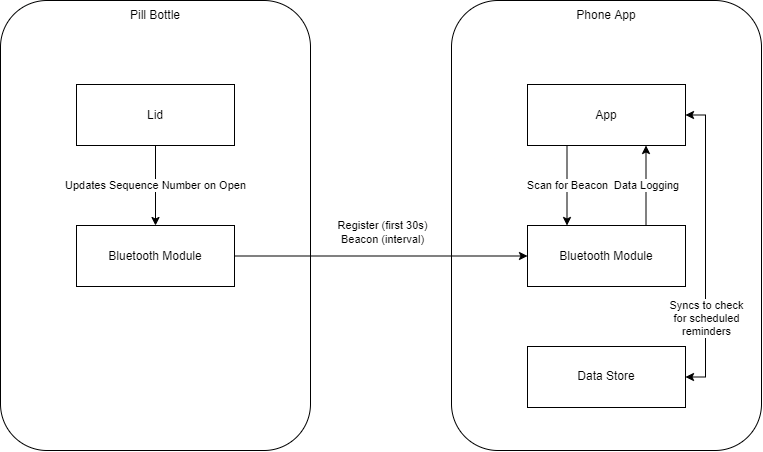
\includegraphics[width=\linewidth]{images/pillpal_block.png}
  \caption{PillPal High Level Block Diagram}
  \Description{A block diagram describing how the PillPal bottle sends data to the PillPal app}
  \label{fig:high_block}
\end{figure}

Figure \ref{fig:high_block} describes how our bottle sends data to the PillPal app. At a high level, a PillPal bottle manages a sequence number representing the number of times the bottle has been opened and advertises it regularly. The app uses received sequence numbers to determine the number of doses taken, and logs any detected dose events. This data can then be used to trigger dosage reminders and low medication notifications. Section \ref{sec:operation} describes the communication protocol in more detail.

\subsection{Theory of Operation}
\label{sec:operation}
PillPal uses Bluetooth Low Energy (BLE) to send data from the bottle to the app. Figure \ref{fig:packet} shows the structure of an advertised PillPal packet.

\begin{figure}[h]
  \centering
  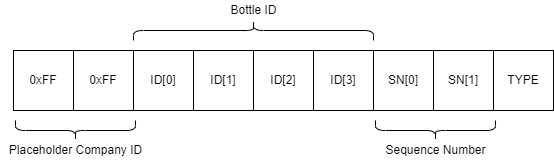
\includegraphics[width=\linewidth]{images/packet.png}
  \caption{PillPal Advertised Packet Structure}
  \Description{A diagram describing the payload of every transmitted PillPall limited discovery packet}
  \label{fig:packet}
\end{figure}

The value of $TYPE$ determines what purpose this packet serves, when $TYPE = 0$, the packet is a beacon packet, and when $TYPE=1$ the packet is a register packet.

Because there is not any data that needs to be streamed, we use a one-way communication protocol, where the PillPal bottle maintains and communicates a state to the app, which then interprets the number of doses taken and total number of pills in the bottle. This simple communication scheme has the benefit of using very little power, but at the cost of not having as much functionality. By not communicating anything to the bottle we lose the ability to have bottle-based audio/visual dosage reminders.

With the communication details out of the way, here are a few in depth description of operations:

\subsubsection{Detecting a Dose}
The PillPal bottle is equipped with a LM393 light sensor module. This light sensor module sends a HIGH signal when it is in the dark, and LOW when it is exposed to light. So, we equate a LOW signal to a bottle opening. An interrupt service routine is attached to this signal, and will increment the bottle's sequence number every time it reads the bottle is opened. This design decision is an easy way to tell if the bottle is open, but also leaves some room for false positives, as light sensors can be very sensitive. This strategy also has the side effect of making our bottle useless in the dark, but we figured that not many users would try to take medication in complete darkness.

\subsubsection{Registering a Medication}
As previously outlined, PillPal uses a one-way communication scheme, so the phone never actually connects to the bottle. Instead, PillPal gives the illusion of connecting to a bottle by having each bottle exclusively send register type packets for the first 30 seconds they are on. The PillPal app is only able to register a new medication if it is able to detect a register type packet in flight it has never seen before.

While the app searches for a register packet in the background, the user is able to enter in information about their medication. This includes the medication name, dosage times, and notification settings. If the app is able to find a new register type packet, the user will have successfully registered a new bottle, and dosage notifications are scheduled. If the app is unable to find a new register type packet, the user will not be able to track a new medication.

\subsubsection{Dosage History}
As outlined in Section \ref{sec:overview}, dosage history is comprised of dosage events. Dosage events are detected when there is a change in sequence numbers in beacon type packets. Sequence numbers are updated via an interrupt triggered when the bottle opens. Dosage events are logged by the app and can be accessed by the user on the medication information screen.

\subsubsection{Dosage Reminders and Notifications}
Upcoming dosage notifications are set up when a medication is registered or modified by the user. The app will periodically check the time, and will send a notification alerting the user of an upcoming dosage within the next 5 minutes. If the user does not take their medication within 5 minutes of the registered time (signaled by an unchanging sequence number), the app will then send a notification alerting the user of a missed dosage. This missed dosage reminder can be extended to contact a healthcare provider or loved one.

\subsubsection{Bottle Location}
Users can request to locate a medication through the medication info screen. The location service will start listening for packets coming from the medication's bottle id, and will use received packet's (Received Signal Strength Indicator) RSSI values to communicate to the user if they are close or far to the bottle.

\subsubsection{Bottle Left Behind Alert}
Users can choose to get alerts if they become separated from any of their medications. When a medication has left behind notifications enabled, the Bluetooth scanning service will record the last time it has seen a packet from the medication's bottle, and will trigger an alert if 1 minute goes by with no received packet from the bottle.

\subsection{Hardware}
\subsubsection{Physical Bottle}
\begin{figure}[h]
  \centering
  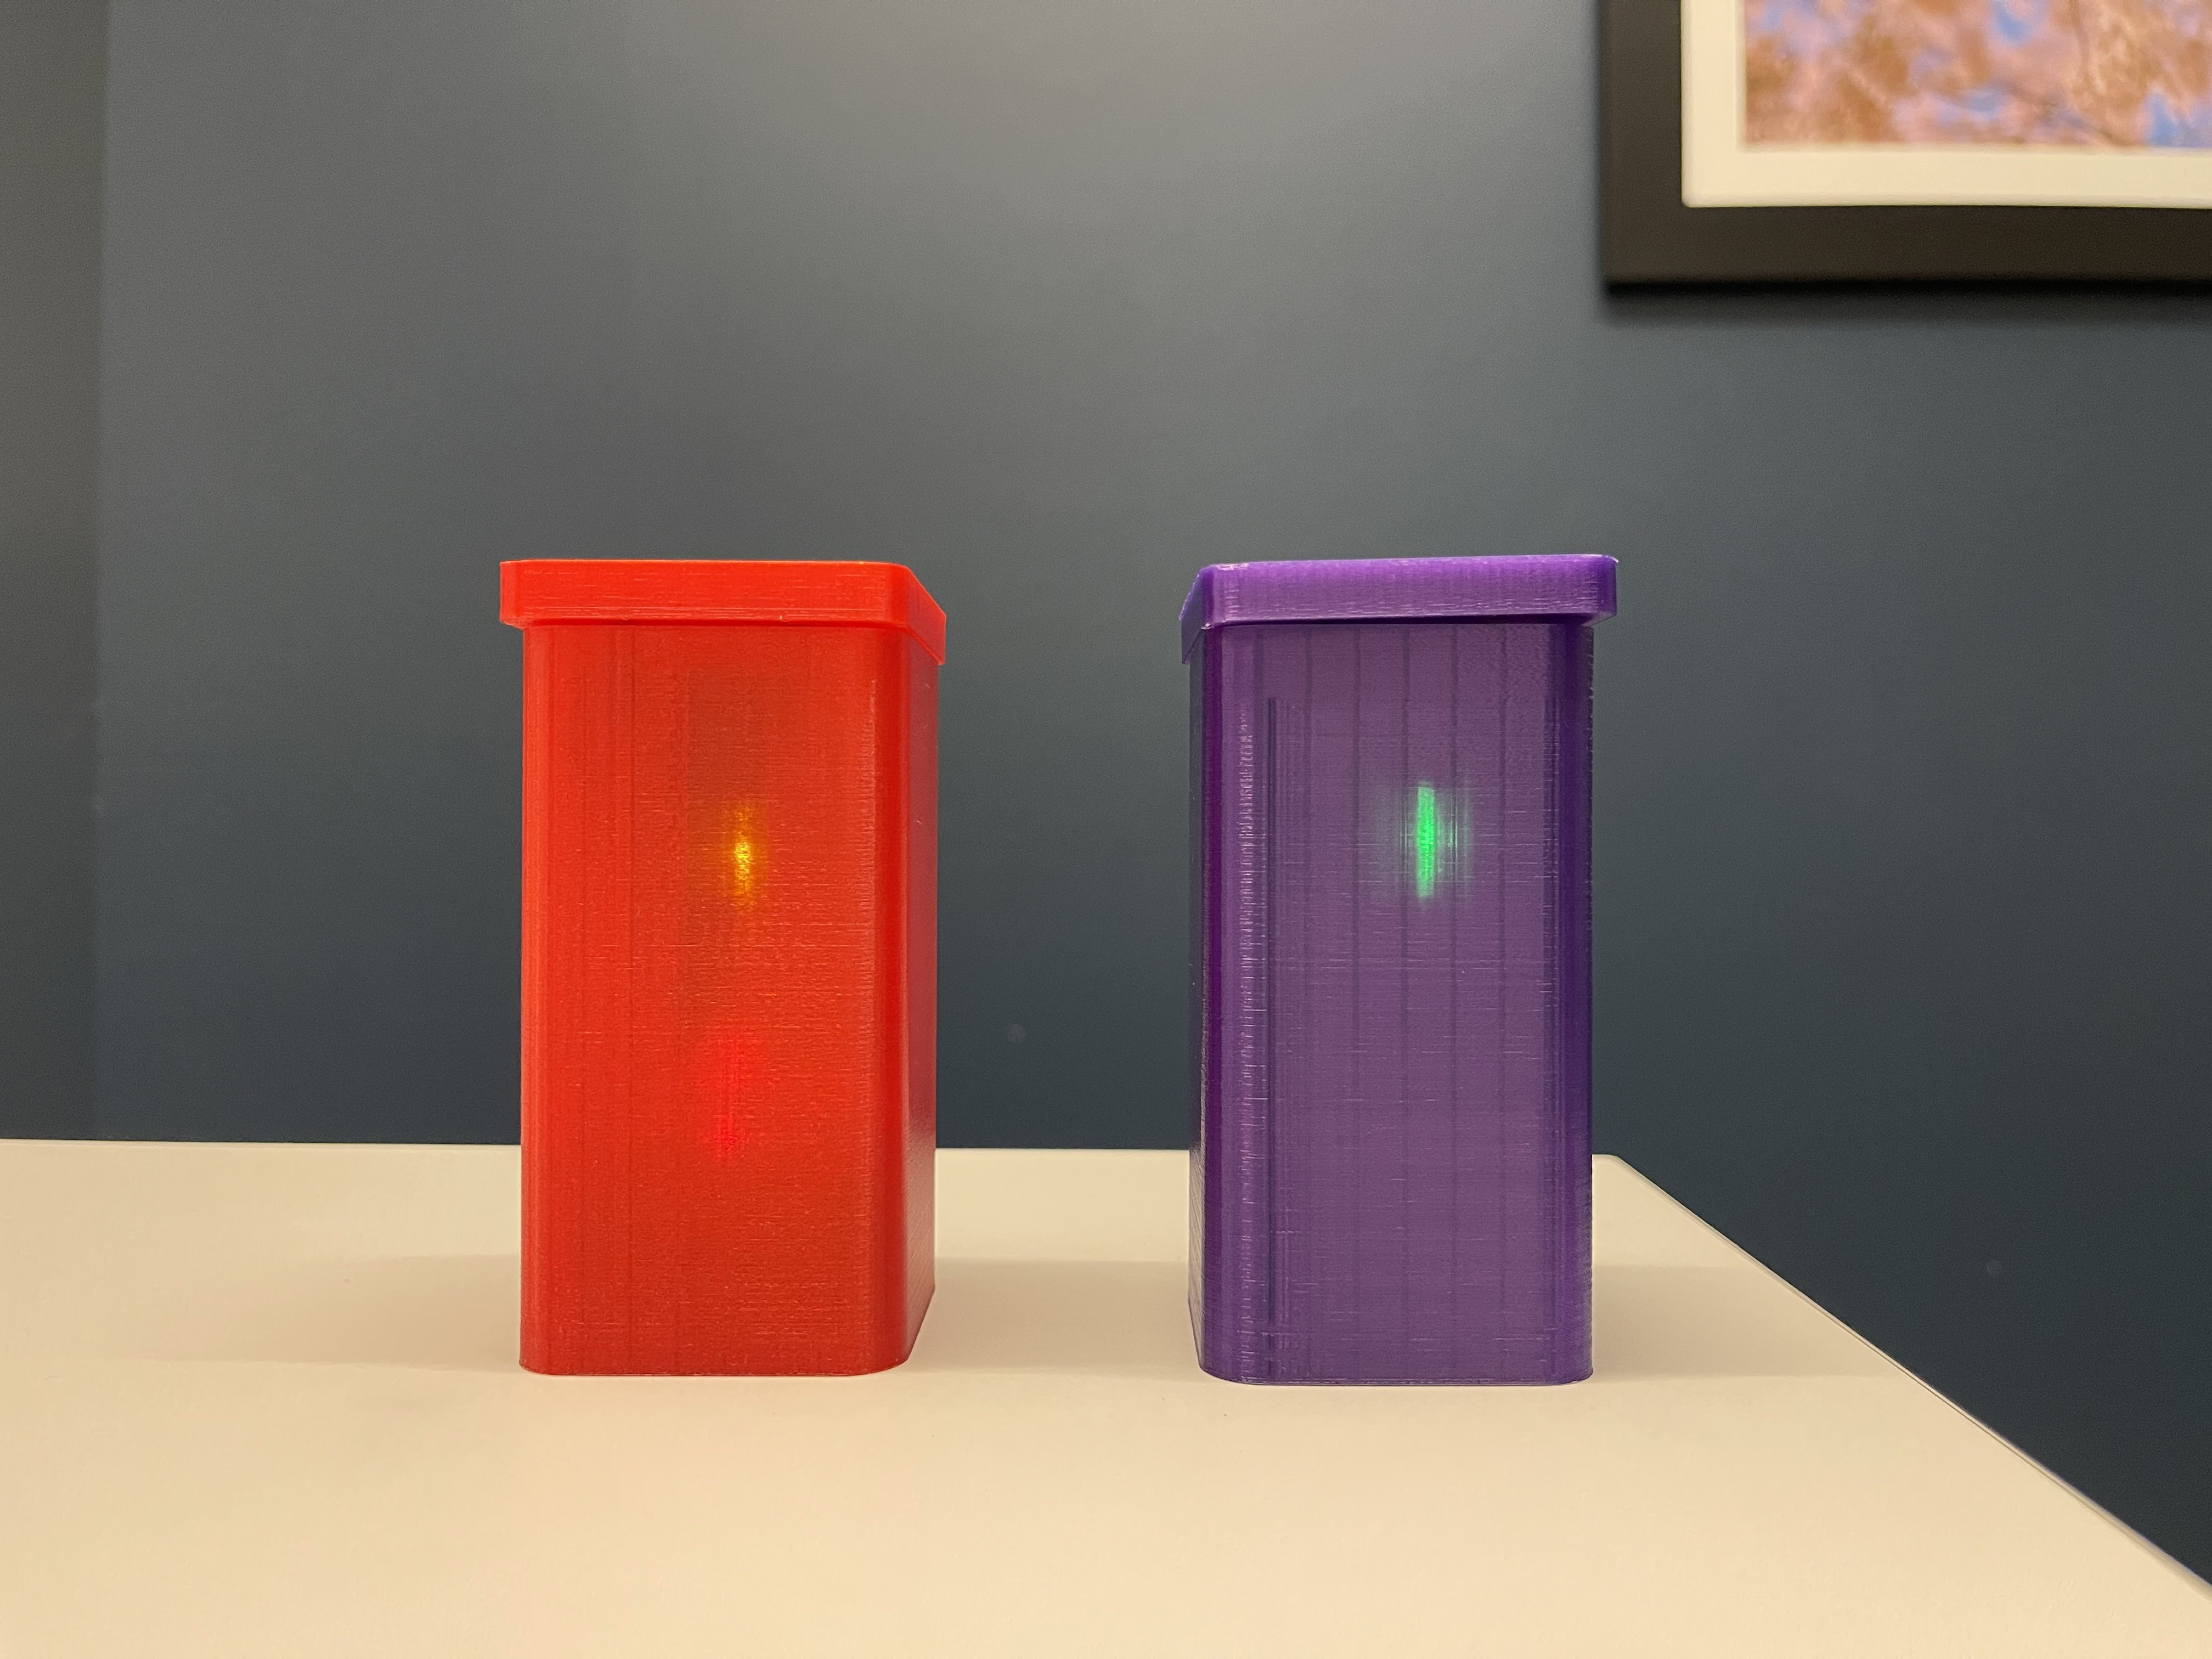
\includegraphics[width=\linewidth]{images/bottle_front.jpg}
  \caption{PillPal Bottles}
  \Description{1 Red PillPal bottle and 1 Purple PillPal bottle. Both are closed.}
  \label{fig:bottle_front}
\end{figure}

The physical PillPal bottle consists of a 3D printed PLA casing, with an electronics chamber and a pill chamber. The electronics chamber contains our Arduino Pro Mini and NRF24L01+ module, along with wires leading to our light sensor module and LiPo battery. The pill chamber provides a clean, wire-free container for pills.

\begin{figure}[h]
  \centering
  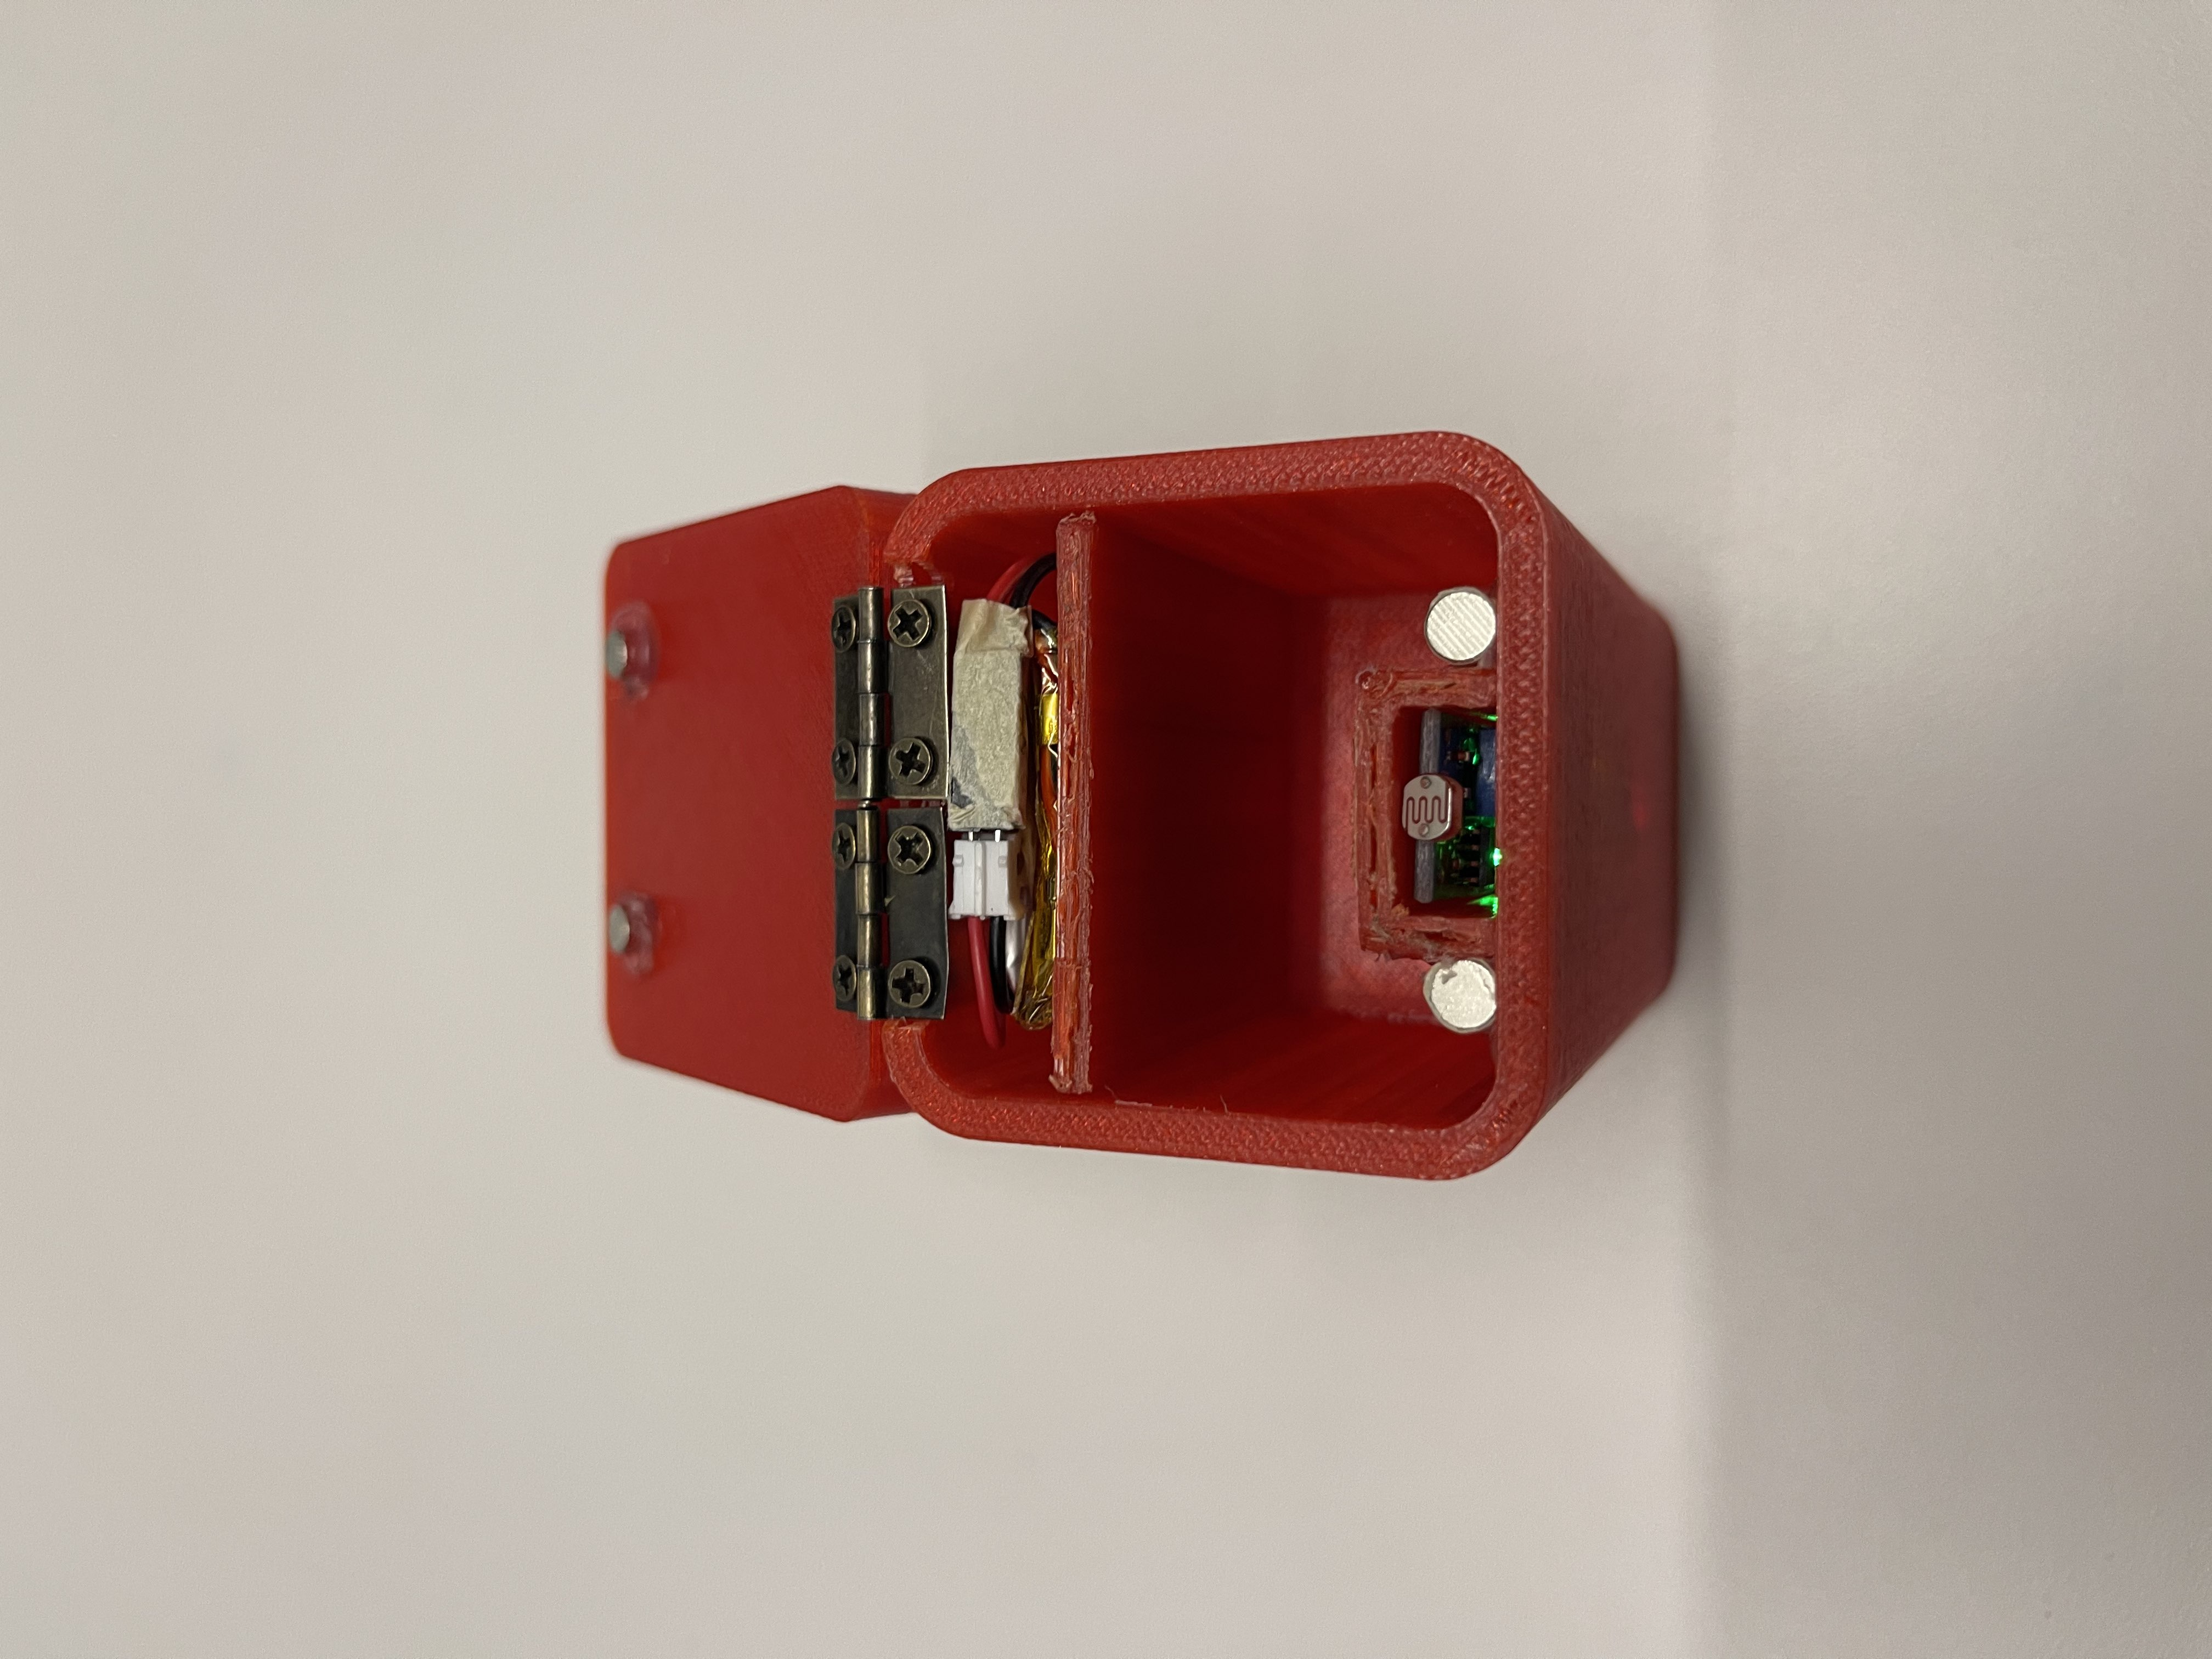
\includegraphics[width=\linewidth]{images/bottle_open.jpg}
  \caption{An open PillPal Bottle}
  \Description{An open PillPal bottle with LiPo battery, light sensor, magnets, and hinges on display}
  \label{fig:bottle_open}
\end{figure}

The bottle's lid is connected by a hinge and held shut with magnets instead of being a twist off cap, as seen in \ref{fig:bottle_open}. This choice was made to make our manufacturing process easier, while still being able to reliably close the bottle.

\begin{figure}[h]
  \centering
  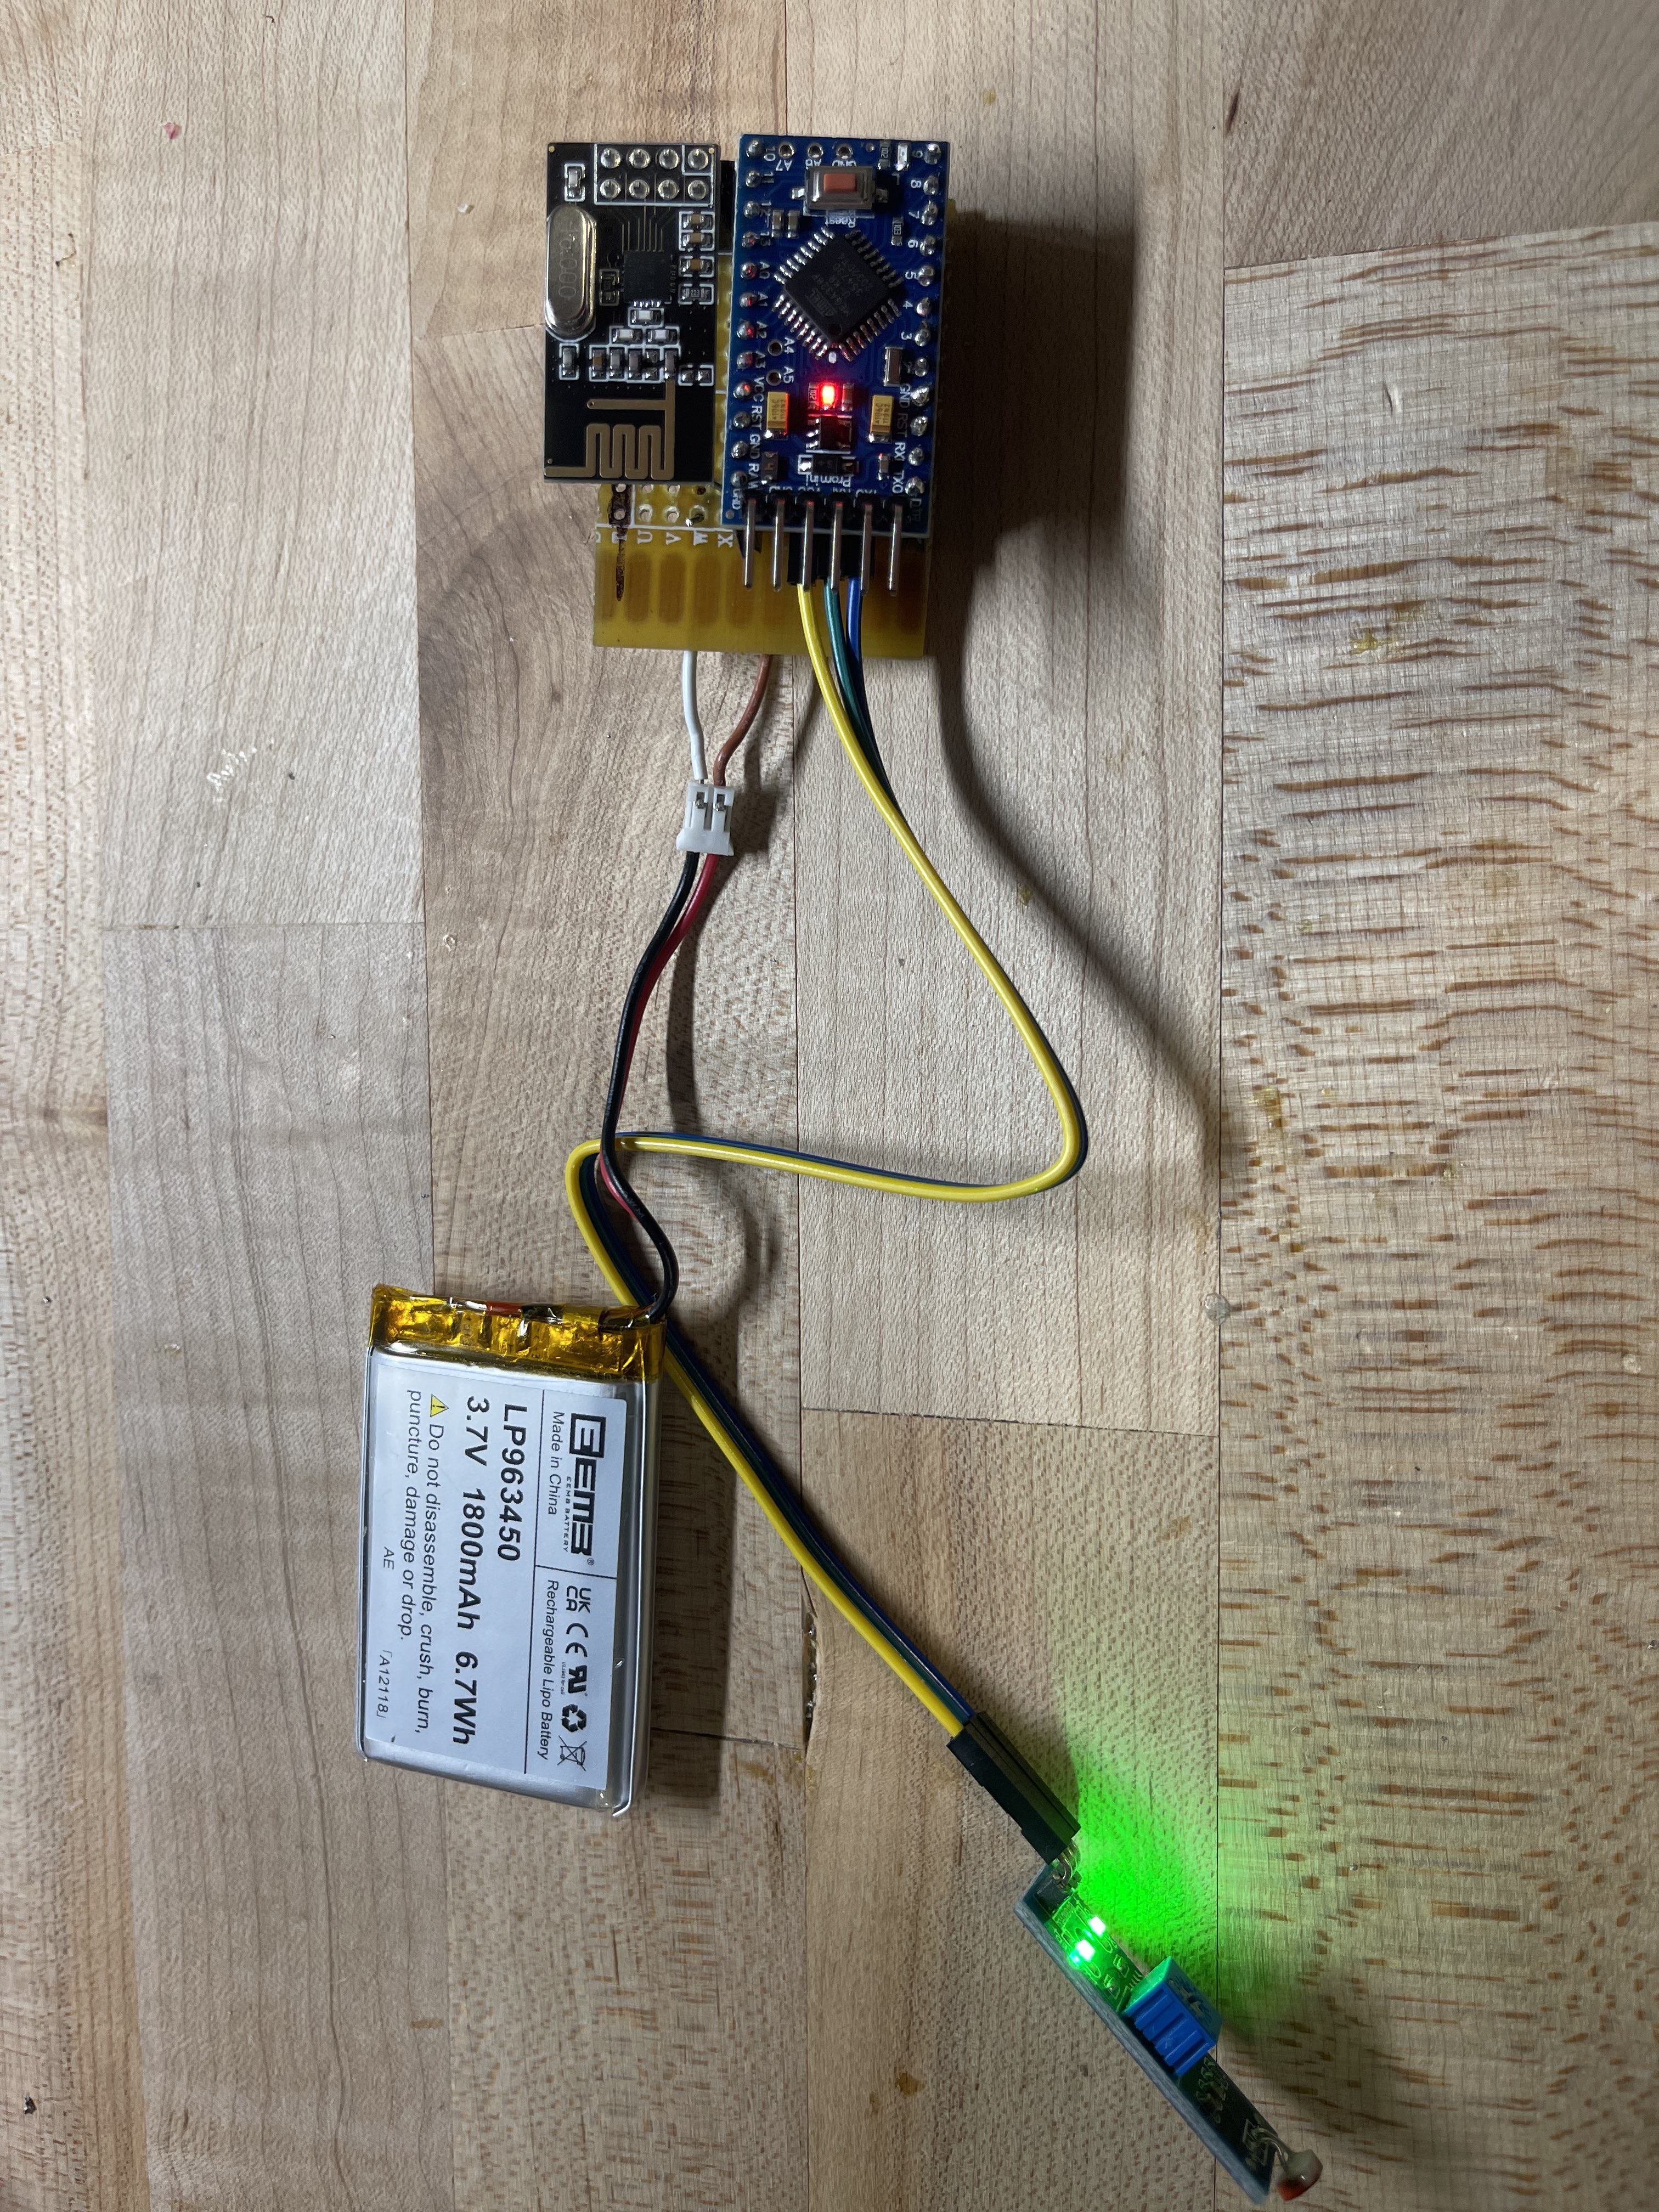
\includegraphics[width=\linewidth]{images/electronics.jpg}
  \caption{Electronic components of a PillPal bottle}
  \Description{MCU and NRF module of PillPal bottle on their breadboard}
  \label{fig:electronics}
\end{figure}

Figure \ref{fig:electronics} shows the electrical components of our bottle. Our Arduino and NRF module are mounted onto a soldered breadboard, which saves clutter from loose wires in the electronics chamber. Wires then lead up into isolated areas along the walls of the pill chamber, and can be seen in \ref{fig:bottle_open}.

\subsubsection{Connection Diagram}
\begin{figure}[h]
  \centering
  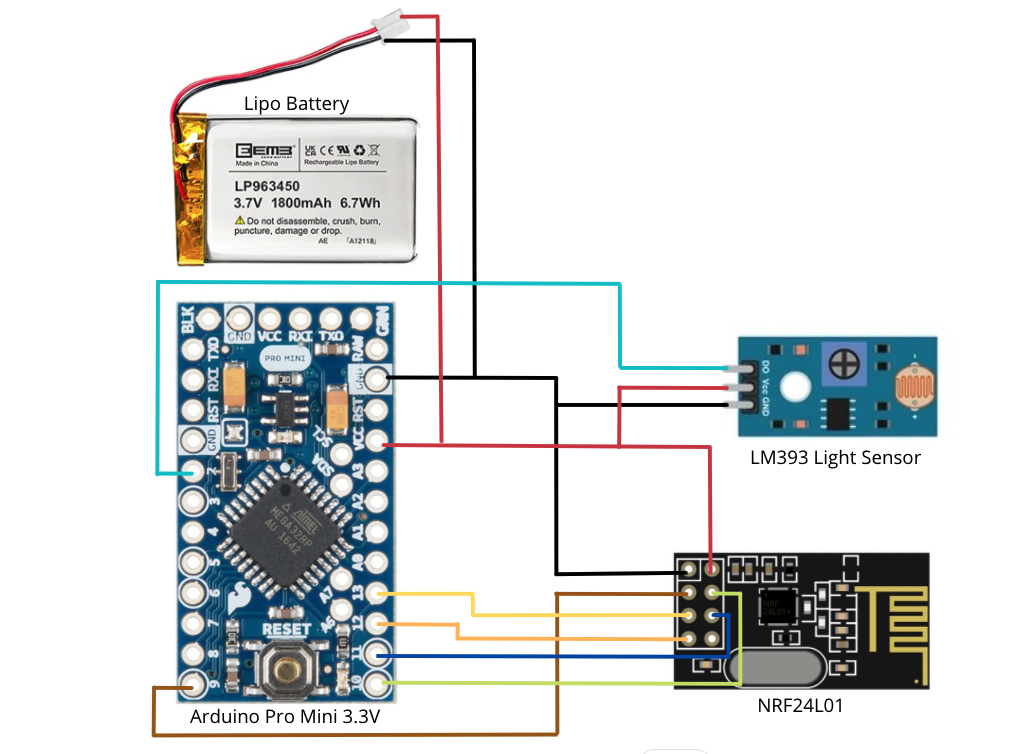
\includegraphics[width=\linewidth]{images/circuit_diagram.png}
  \caption{PillPal Circuit Diagram}
  \Description{Schematic outlining the connections used in the PillPal bottle circuit.}
  \label{fig:circuit}
\end{figure}

Figure \ref{fig:circuit} shows the connections used by our bottle. The electronics in the PillPal bottle are all powered by a 3.7V 1800mAh LiPo battery, which connects directly to an Arduino Pro Mini. The Arduino's 3.3V output pin is used as a voltage regulated power supply for both the light sensor and NRF modules. Power calculations are discussed in Section \ref{sec:power_calc}.

\subsection{Software}
\subsubsection{Embedded Architecture}
\label{sec:embeded_arch}
\begin{figure}[h]
  \centering
  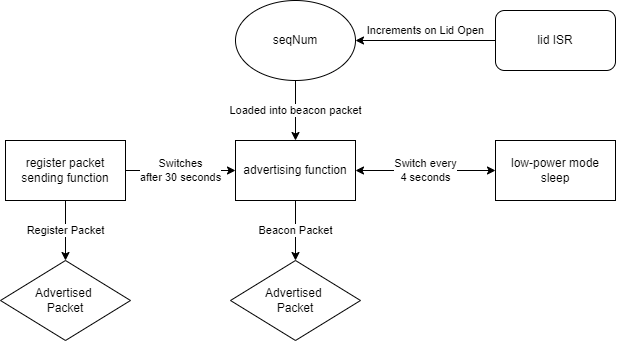
\includegraphics[width=\linewidth]{images/embedded_block.png}
  \caption{PillPal Embedded Code Block Diagram}
  \Description{PillPal Embedded Code Block Diagram, describes data flow.}
  \label{fig:em_block}
\end{figure}

Our MCU code (diagrammed in Figure \ref{fig:em_block}) is  optimized for power saving - there is very little computation done on the bottle's Arduino. For the first 30 seconds after power on, the bottle will only advertise register packets, and then switch into normal operation mode. In normal operation mode, a lid open interrupt is set and the controller will switch between an advertising function and sleeping in low-power mode every 4 seconds.

The lid open ISR is triggered whenever the bottle's light sensor is exposed to light, which signals the lid is open and the user is taking a dose.

We chose a 1:1 duty cycle of because the app scans for Bluetooth packets every 6 seconds. This 4 second duty cycle guarantees that at least one packet from the bottle will be in flight every 2 scans from the app. This gives a good balance of performance and power savings, as the other options are to make the app accept potentially longer latencies, or make the bottle constantly advertise packets.

\subsubsection{App Architecture}
\label{sec:software_arch}
\begin{figure}[h]
  \centering
  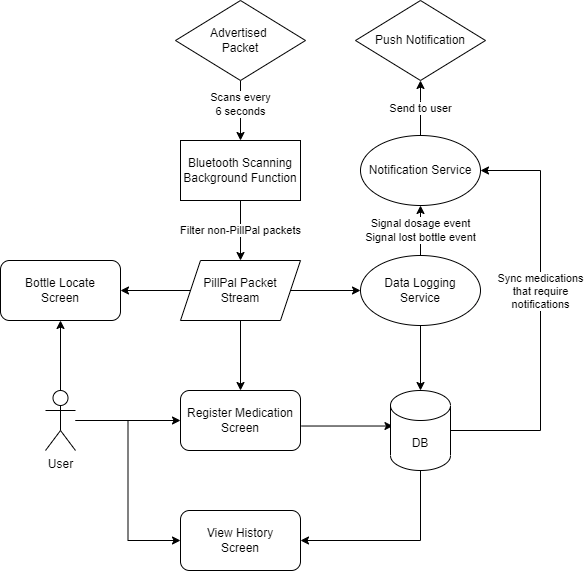
\includegraphics[width=\linewidth]{images/app_block.png}
  \caption{PillPal App Code Block Diagram}
  \Description{PillPal App Code Block Diagram, describes data flow.}
  \label{fig:sw_block}
\end{figure}

The core component of the app is a Bluetooth scanning service which is constantly running, even when the app is closed. We accomplish this by creating a service notification and run our app code as a foreground process. This scanning service will read all BLE packets available, and filter out PillPal packets to a global packet stream.

This PillPal packet stream can then be used by the backend data logging service, or by the user screens which need Bluetooth information (RSSI-based locator and medication registration). The backend data logging service processes the incoming PillPal packets by examining the senders and sequence numbers. If the backend data logging service detects any events, it sends the notification service a request to display a push notification to the user.

\section{Evaluation and Results}
PillPal has yet to see any real world use - it has only been used in testing periods held multiple hours at a time.

\subsubsection{Power Use}
\label{sec:power_calc}
We estimate that our bottle is able to run for up to 10 days on one single charge. We found this estimate by measuring the current of our microcontroller in both advertise and low-power mode:

\begin{align*}
  A_{advertise} = 9mA && A_{low-power} = 6mA
\end{align*}

We run a 1:1 duty cycle of advertise mode to low-power mode, so our average current is
\begin{align*}
  A_{avg} = 7.5mA
\end{align*}

Considering our battery's capacity of 1800mAh, this means our maximum run time is
\begin{align*}
  \frac{1800mAh}{7.5mA} = 240. hours = 10. days
\end{align*}

Similarly lightweight Bluetooth devices often last up to a year, so while this is a great start there is certainly room to improve.

\subsubsection{Production Cost}
\begin{table}[]
  \caption{PillPal Bottle Price Breakdown}
  \begin{tabular}{ll}
  Name of Product             & Price   \\
  BLE module: NRF24L01        & $\$1.30$  \\
  LM393 Light Sensor Module   & $\$0.59$  \\
  3.7V 1800mAh LiPo Battery   & $\$12.99$ \\
  Wiring Materials            & $\$2.26$  \\
  Arduino Pro Mini            & $\$5.33$  \\
  Mini Hinges                 & $\$0.32$  \\
  Magnets                     & $\$0.14$  \\
  PLA                         & $\$2.65$  \\
  Misc. (solder, tape, wires) & $\$0.50$  \\ \hline
  Total                       & $\$28.74$
  \end{tabular}
  \label{Tab:price_breakdown}
\end{table}

We identify the cost of the production of one bottle in table \ref{Tab:price_breakdown}. The most expensive materials are the LiPo battery and Arduino Pro Mini. A possible next step in reducing our production cost could be switching our MCU to an arm M0 based device, possibly on our own PCB. Our microcontroller does very little computation so we do not need most of the features an off-the-shelf MCU has.

That being said, existing smart bottles can are sold in the \$40+ range. Our bottle can already be sold below that margin, and would likely become cheaper if we were to scale up its production.


\section{Discussion}
While we are proud of the work and design that went into PillPal, we acknowledge that our work has its fair share of flaws.

\subsection{Future Work}
Two easily identifiable areas of improvement are battery life and app over-reliance.

Similar devices such as the Tile use coin cell batteries for power, but are able to run for up to a year without replacement \cite{tile}. The Tile does a similarly small amount of computation as our MCU, so one logical next step could be to closely investigate how the Tile manages its power and incorporate those ideas into our own power management.

Another area of improvement is our app over-reliance. Almost all our functionality is contained in our app, taking away all the "smart" features of the bottle if not near the phone. We would like to add visual/audio cues to our bottle and a sensor or set of sensors which can signal when the bottle is empty or low on medication.

\subsection{Lessons Learned}
As a team, we all got to learn a lot about app development with Flutter, working with Bluetooth packets, and designing Arduino code with interrupts.

We'd like to use this space to reflect and discuss what we learned individually, as well.

\textbf{Alex:} For technical knowledge, I learned about app development with the Flutter Framework. It was not something I had done before and took some adjustment to get going. I also sharpened my teamwork skills.

\textbf{Peter:} I learned the importance of project management. I acted as a project manager for the first few weeks of the quarter, but I was inactive for a few weeks in the middle of the quarter, and as a result I think the team had a lack of direction until the week before the final presentation. At the very least I'm thankful to know I don't want to be a project manager at this point in my career. :')

\textbf{Sunny:} I learned about how important it is to clearly communicate the expectations and goals of a project, especially at the start of the project. The PRD allowed us to narrow down what we wanted to accomplish in the project, but we encountered some issues during development where one goal was achieved but also made accomplishing another goal more difficult. In the future, I'd advocate for more detailed milestones.

\textbf{Edward:} In terms of knowledge, I learned a lot about Bluetooth and how to choose the right hardware to solve a practical problem. Besides that, one important lesson I learned is that to complete one thing, we need to constantly find and solve problems, which is reflected in our development process all the time. However, I should think more carefully when considering the initial plan in the future, to reduce unnecessary costs. For example, I did not compare the energy consumption of different microprocessors well enough at the beginning which caused us to pick the option with a relatively high energy consumption. 

\section{Conclusion}
We have presented PillPal, a simple medication organizer. We hope that we have presented a system that, with some more polish, seems feasible to use in the real world - even if only for convenience in remembering to take medication.

%%
%% The next two lines define the bibliography style to be used, and
%% the bibliography file.
\bibliographystyle{ACM-Reference-Format}
\bibliography{pillpal}

\end{document}
\endinput
